Programming for SIEMENS Tecnomatix Process Simulate was initially desirable, as it exposes a Microsoft .NET Framework compatible API. This allows developers to choose any of the many .NET languages to create Process Simulate plugins, including but not limited to C\#, C++, F\#, Visual Basic, Iron Python. All the code in this work is written in C\#.

\section{Writing Plug-ins}
Any .NET assembly can be a Process Simulate plugin, as it only looks at the contents. 
A class library project is ideal for this as there is no benefit for any other project type. 
For Process Simulate to pick up the assembly, it should be located in \emph{DotNetCommands} or \emph{DotNetExternalApplications} directories and registered with the application. 
These directories and any following paths are relative to the programs installation directory. 
Typically this would be \cls{C:/Program Files/Tecnomatix 13.0/eMPower}, but might differ based on the user's choice at install-time.

To register an external application or a command with Process Simulate, we need to use a utility \emph{CommandReg.exe} which comes with the application. When you launch the program a dialog, similar to the one presented in Figure \ref{fig:CommandReg}, will appear. In this dialog we select the compiled file, we want to load, pick the commands located in the assembly and choose a filename for the configuration XML file which will be newly created. This XML allows the settings to be moved between computers easily. \\

\begin{figure}[H]
    \caption{CommandReg Utility}
    \centering
    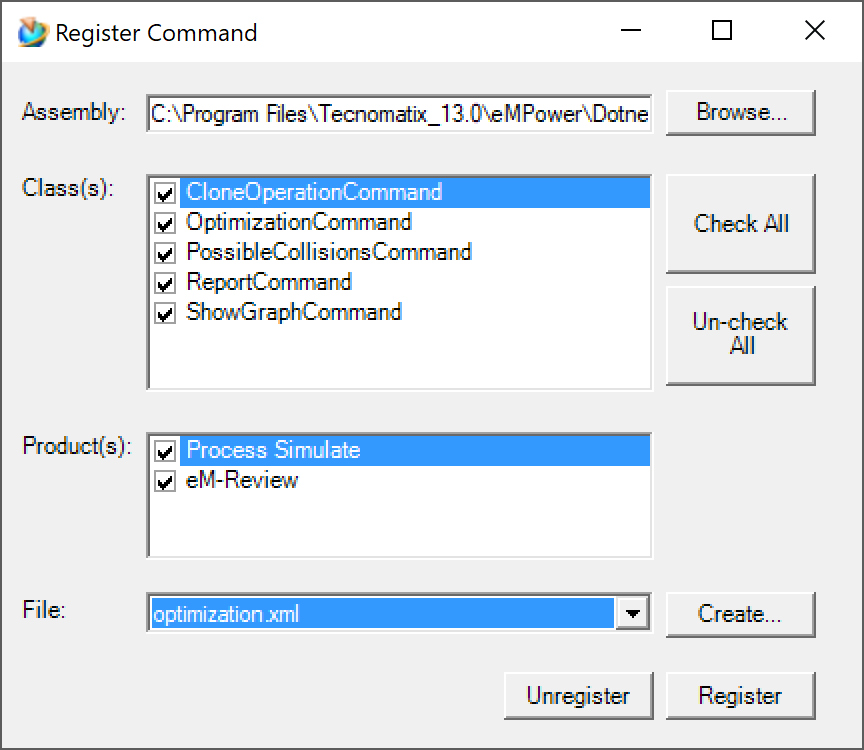
\includegraphics{commandreg}
    \label{fig:CommandReg}
\end{figure}

After we registered our commands, we need to configure our workspace to be able to use them. More specifically, we need to choose where the application should display buttons for the commands in the ribbon menu. This can be achieved by right-clicking the ribbon to invoke the context menu and selecting the \emph{Customize Ribbon} option as shown in Figure \ref{fig:CustomizeRibbonContextMenu}. A dialog like you see in Figure \ref{fig:CustomizeRibbonDialog} will appear where the user can add new commands to the ribbon and customize the layout. The newly registered actions will appear in the list. Unfortunately, there is no grouping available. Therefore the best option is to look for the exact names in the alphabetically sorted list.

\begin{figure}[H]
    \caption{Customize the Ribbon}
    \centering
    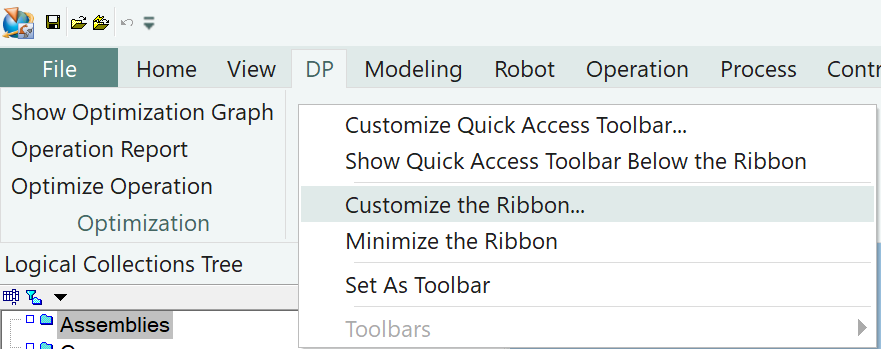
\includegraphics{customizeribbon}
    \label{fig:CustomizeRibbonContextMenu}
\end{figure}

\begin{figure}[H]
    \caption{Add commands to the Ribbon}
    \centering
    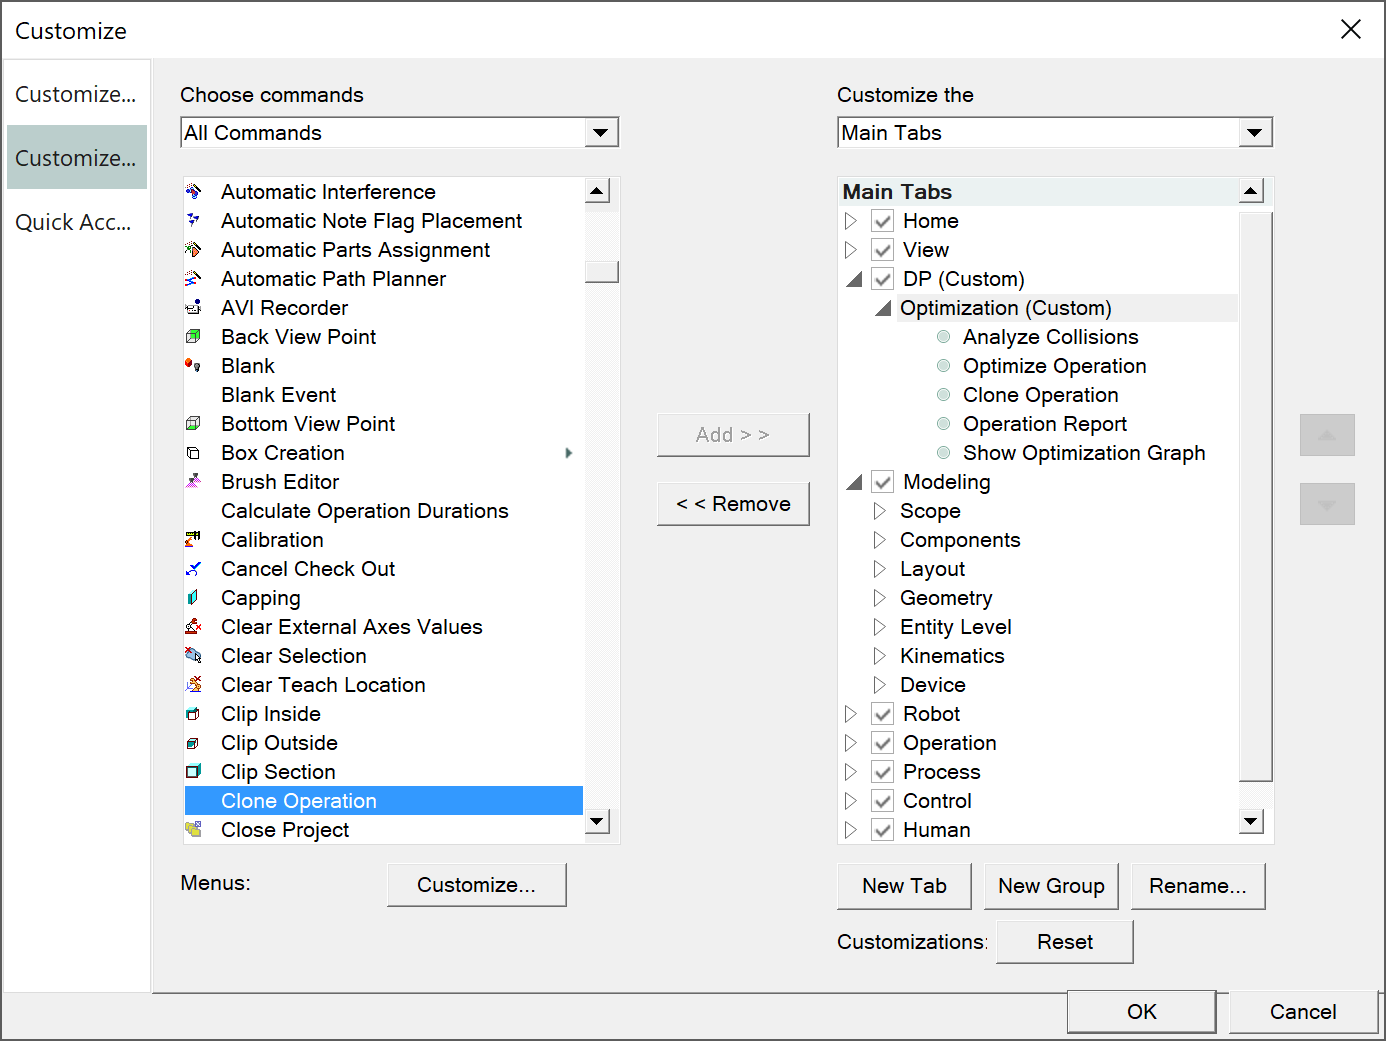
\includegraphics[width=\textwidth]{addcommands}
    \label{fig:CustomizeRibbonDialog}
\end{figure}

Next, we will look like at how to code new commands so that Process Simulate would recognize them. For this, we first need to include a reference for the main dynamically linked library \namespace{Tecnomatix.Engineering.dll}. Writing plugins for the application revolves mostly around this one library, as it contains all the classes used to interact with the application.

\begin{figure}[H]
    \caption{Example Command}
    \centering
    \begin{minted}{csharp}
public class MyCommand : TxButtonCommand
{
    public override String Category { get; } = "My Category";
    public override String Name { get; } = "My Command";
    public override void Execute(Object cmdParams)
    {
    }
}
    \end{minted}
    \label{fig:CodeCommand}
\end{figure}
